\documentclass[aspectratio=169, 12pt, a4paper, hyperref={pdfauthor={Alexandre MARIN}, pdfkeywords={IFPEN, Delaunay, Voronoi, mesh generation}, colorlinks=true, linkcolor=purple, urlcolor=blue, citecolor=magenta}]{beamer}
\usepackage[utf8]{inputenc}
\usepackage[french]{babel}
\usepackage[T1]{fontenc}
\usepackage{amsmath}
\usepackage{amsfonts}
\usepackage{amssymb}
\usepackage{graphicx}
\usepackage{xcolor}
\usepackage{tikz}

\usepackage[francais]{IFPENPresentation}
\usepackage{array}
\usepackage{multirow}
\usepackage{ctable}

\usepackage[defaultbib]{bibtopic}
%\renewcommand{\thesection}{\arabic{section}}

\graphicspath{{figures/}{pictures/}}



\begin{document}

\begin{frame}
\institute[]{
IFP \'Energies nouvelles\\ 
Direction Sciences et Technologies du Numérique -- Département Informatique Scientifique\\
1-4 avenue du Bois-Préau \textsc{RUEIL-MALMAISON}}
\date{2 novembre 2020}
\author{\small Alexandre \textsc{MARIN}\\ { Master Mathématiques et Applications Sorbonne Université\\ Parcours Ingénierie Mathématique\\ Majeure Ingénierie Mathématique Pour l'Entreprise}}
\title{Développement d’une bibliothèque de structures et algorithmes pour un mailleur polyédrique}
\subtitle{\small Soutenance de fin de stage\\ Encadrants :\\ Laurent \textsc{Astart}, Alexandra \textsc{Bac}}
\maketitle
\end{frame}

\begin{Energie}{Plan}
\tableofcontents
\end{Energie}

\section{Introduction}

\subsection{Présentation d'IFPEN}
\begin{Energie}{Brève présentation d'IFPEN}
\begin{itemize}
\item un EPIC
\item $\approx 50$\% de son budget issu de l'\'Etat
\item un groupe employant $1\ 600$ salariés
\item conçoit et développe des procédés, équipements et logiciels relatifs à quatre domaines :\setbeamertemplate{items}[square]
\begin{itemize}
\item la mobilité durable
\item les énergies renouvelables
\item les hydrocarbures responsables
\item \textcolor{red}{le climat/environnement}
\end{itemize}
\end{itemize}
\end{Energie}

\subsection{Objectifs}
\begin{Energie}{Objectifs}

Premier objectif : faire un travail bibliographique et développer des structures de données et algorithmes pour un mailleur polyédrique 3D, censé être adapté à la simulation d'écoulements dans le sous-sol.
\\[1cm]
\begin{visibleenv}<2>
Objectif retenu : s'approprier des concepts sur la génération de maillages 2D et mettre en \oe{}uvre certains algorithmes en programmant une bibliothèque logicielle.
\end{visibleenv}
\end{Energie}

\subsection{Calendrier}
\begin{Energie}{Déroulement du stage}
{\renewcommand{\arraystretch}{1.5}
\renewcommand{\tabcolsep}{0.2cm}
\begin{tabular}{c|p{12cm}}
Juillet & Installation, programmation en C++ d'une structure en demi-arêtes et d'algorithmes de génération de maillages Delaunay\\
Août & Réorganisation du code, génération de maillages Delaunay contraints, tests\\
Septembre & Création de diagrammes de Voronoï, rédaction du rapport\\
Octobre & Seconde étude bibliographique\\
\end{tabular}}
\end{Energie}

\begin{Energie}{Contexte}

\begin{visibleenv}<1,4->
La simulation d'écoulements dans le sous-sol nécessite des maillages tels que :
\begin{itemize}
\item<1,4,5,6> les éléments structuraux apparaissent
\item<4-> certaines contraintes géométriques soient respectées\only<4>{ (régularité, conformité, orthogonalité$\dots$)}
\end{itemize}
\end{visibleenv}

\begin{onlyenv}<2>
\begin{center}\vspace{-1cm}
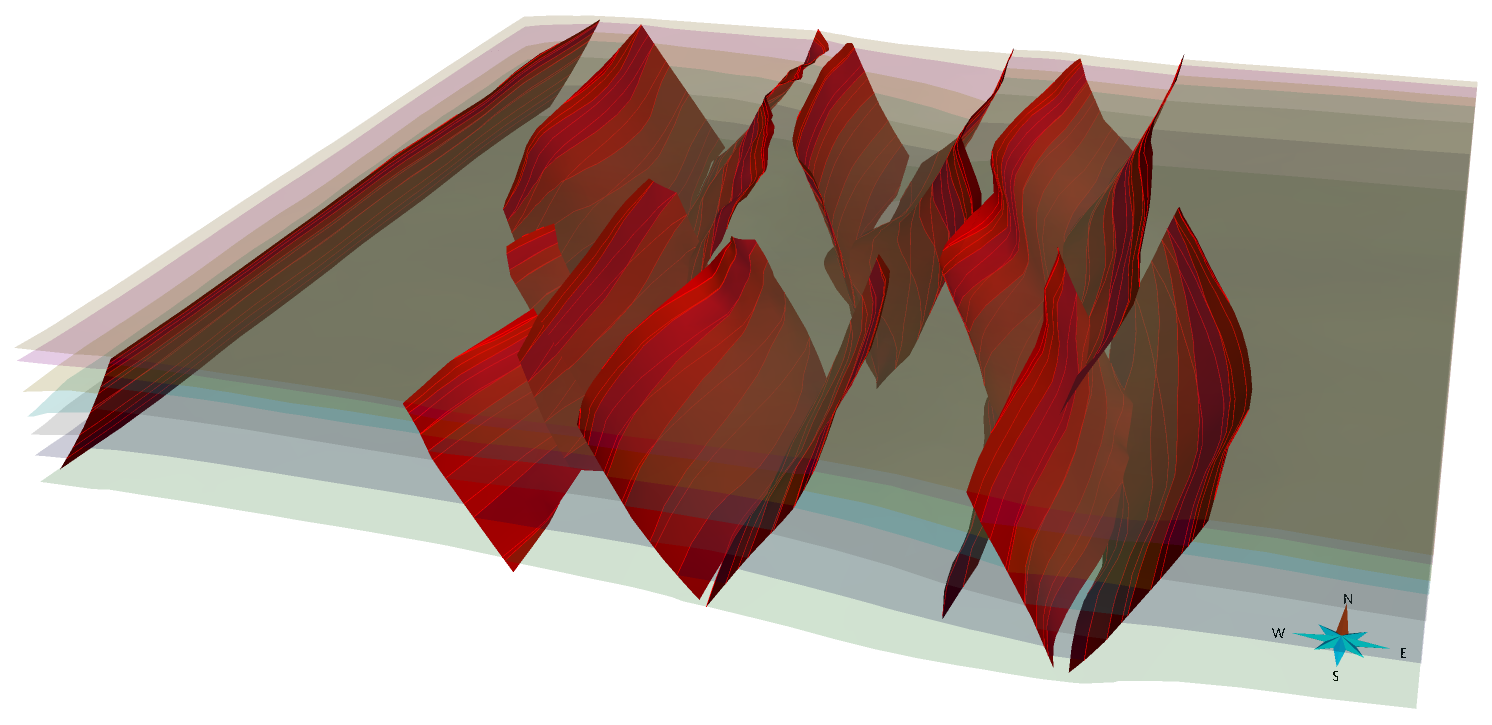
\includegraphics[scale=0.27]{Analog.png}
\\Exemple d'un ensemble d'horizons et de failles à respecter\\(source : \url{https://geoanalog.ifpen.fr/})
\end{center}
\end{onlyenv}
\begin{onlyenv}<3>
\begin{center}\vspace{-1cm}
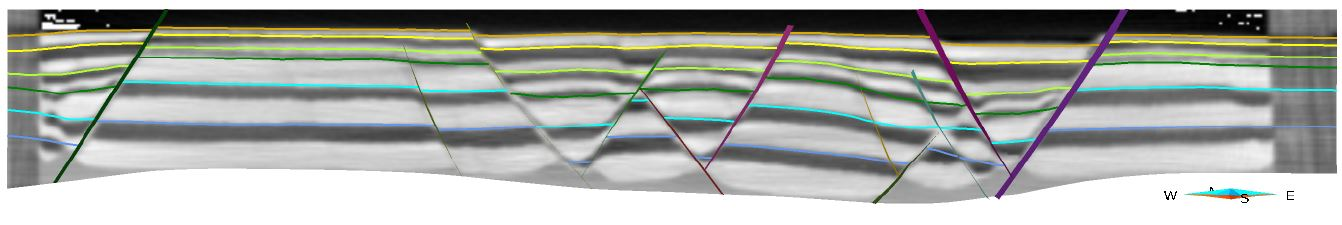
\includegraphics[scale=0.5]{crossSectionClyde.jpg}
\\Une section de ce modèle\\(source : figure 5C de l'article \cite{TERTOIS_RM2020})
\end{center}
\end{onlyenv}

\uncover<5->{\vspace{1cm} Avec des méthodes du type \emph{Volumes finis} ou \emph{\'Eléments virtuels}, il est possible d'utiliser des maillages polyédriques.}

\uncover<6->{\vspace{1cm} Quelles sont les bonnes propriétés de tels maillages vis-à-vis de ces méthodes numériques ?}

\end{Energie}

\begin{Energie}{\small Quelques exemples de domaines géologiques}
\begin{center}
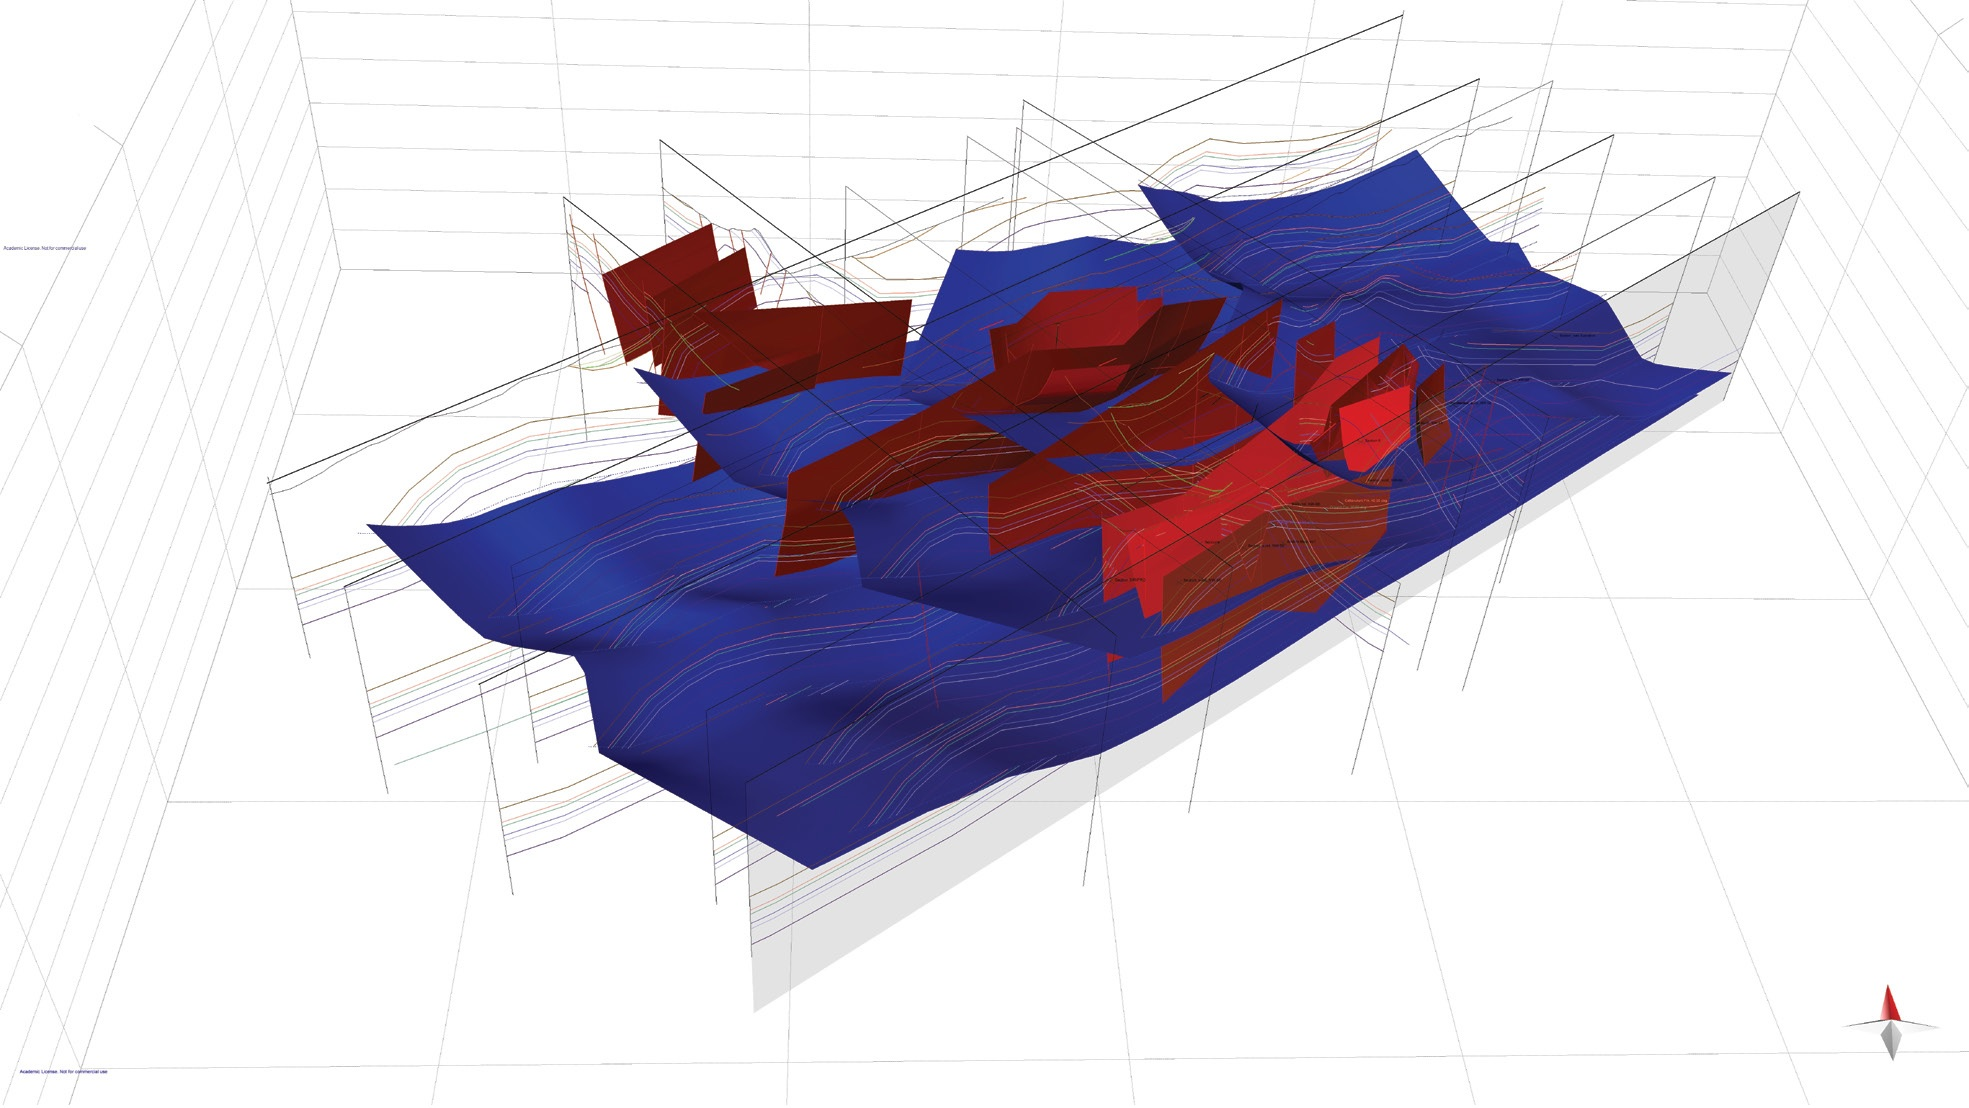
\includegraphics[scale=0.25]{thrusts.jpg}
\\Modèle géologique reconstruit, failles inverses en bleu et failles transpressives en rouge (source : \cite{Sicily})
\end{center}
\end{Energie}

\begin{Energie}{\small Quelques exemples de domaines géologiques}
\begin{center}
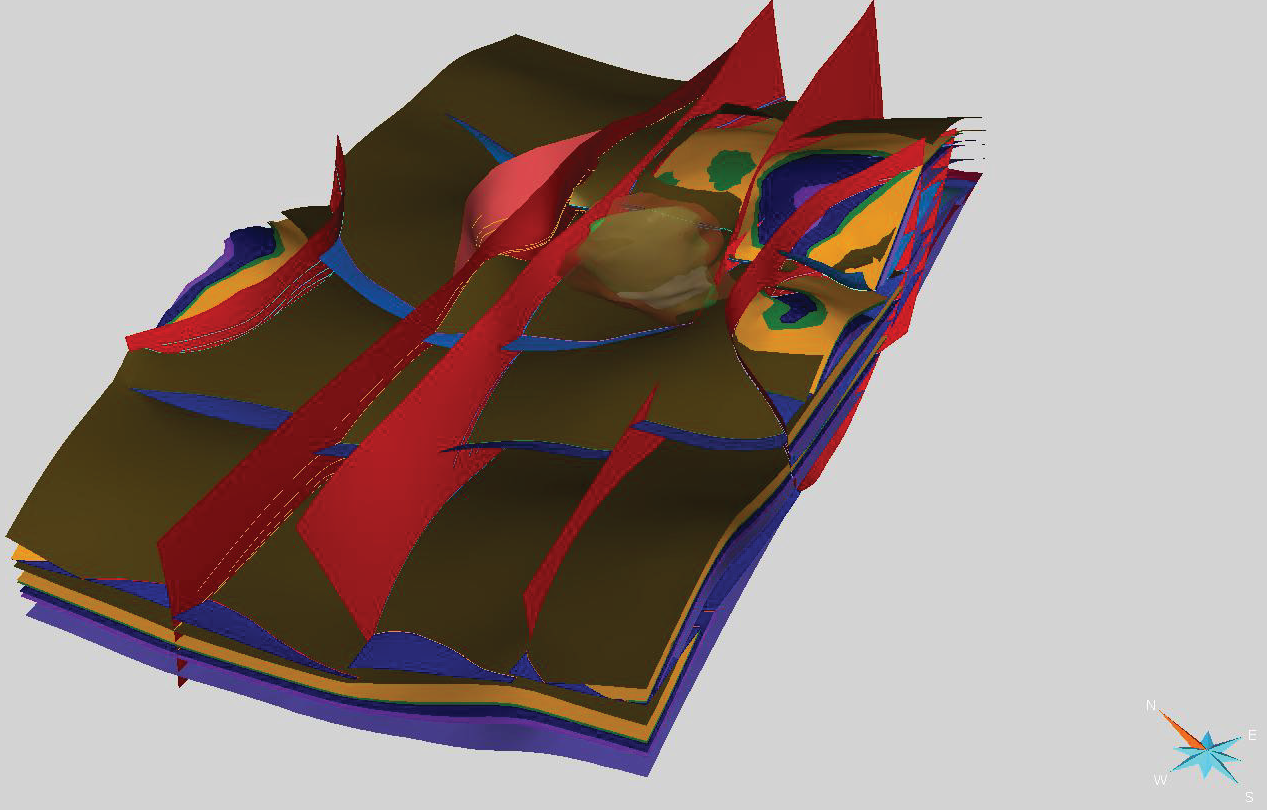
\includegraphics[scale=0.35]{thrustsHorizons.png}
\\Modèle géologique reconstruit précédent, avec les horizons (source : \cite{Sicily})
\end{center}
\end{Energie}

\begin{Energie}{\small Quelques exemples de domaines géologiques}
\begin{center}
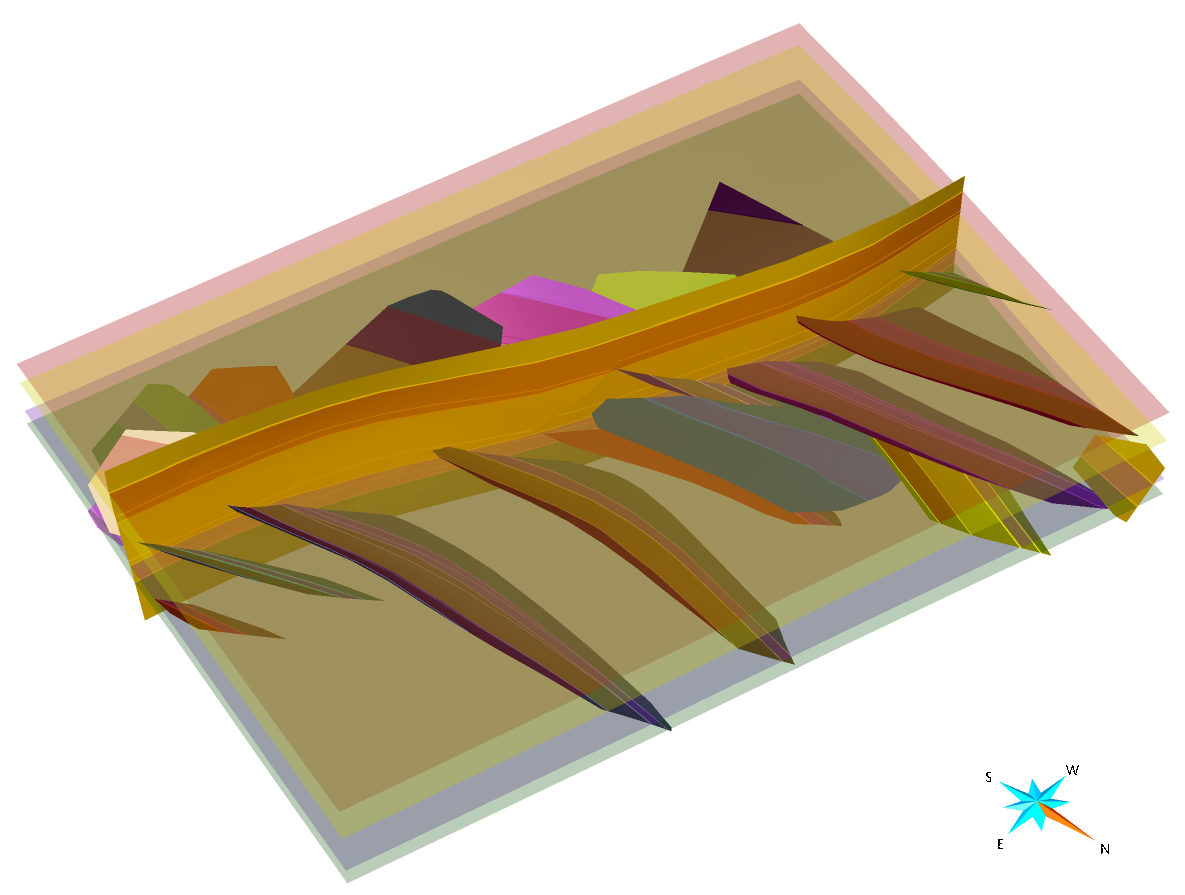
\includegraphics[scale=0.25]{Clyde.png}
\\Une faille principale décrochante, quelques failles de part et d'autre de celle-ci (source : \cite{TERTOIS_RM2020})
\end{center}
\end{Energie}


\section{Mission du stage}
\begin{Energie}{}
\tableofcontents[currentsection]
\end{Energie}

\begin{Energie}{Triangulation de Delaunay}
\begin{center}
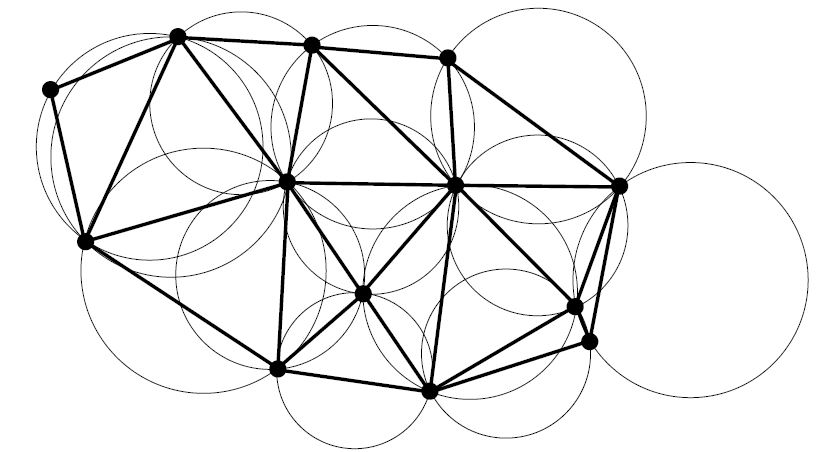
\includegraphics[scale=0.55]{../pictures/delTri.jpg}
\\figure 2.3 de la source \cite{delnotes}
\end{center}
\end{Energie}

\begin{Energie}{Diagramme de Voronoï}

Pour un ensemble fini $S\subset\mathbb{R}^2$, c'est une famille de convexes polyédriques $(V_{p})_{p\in S}$ recouvrant le plan :
\[V_p\ :=\ \left\{x\in\mathbb{R}^2\middle\vert\ \forall\,q\in S,\ \Vert x-p\Vert\leqslant\Vert x-q\Vert\right\}\text{.}\]
\end{Energie}

\begin{Energie}{Dualité Delaunay/Voronoï}
\vspace*{-1cm}Triangulation de Delaunay en bleu,
arêtes du diagramme de Voronoï en blanc\\[0.8cm]
\begin{center}
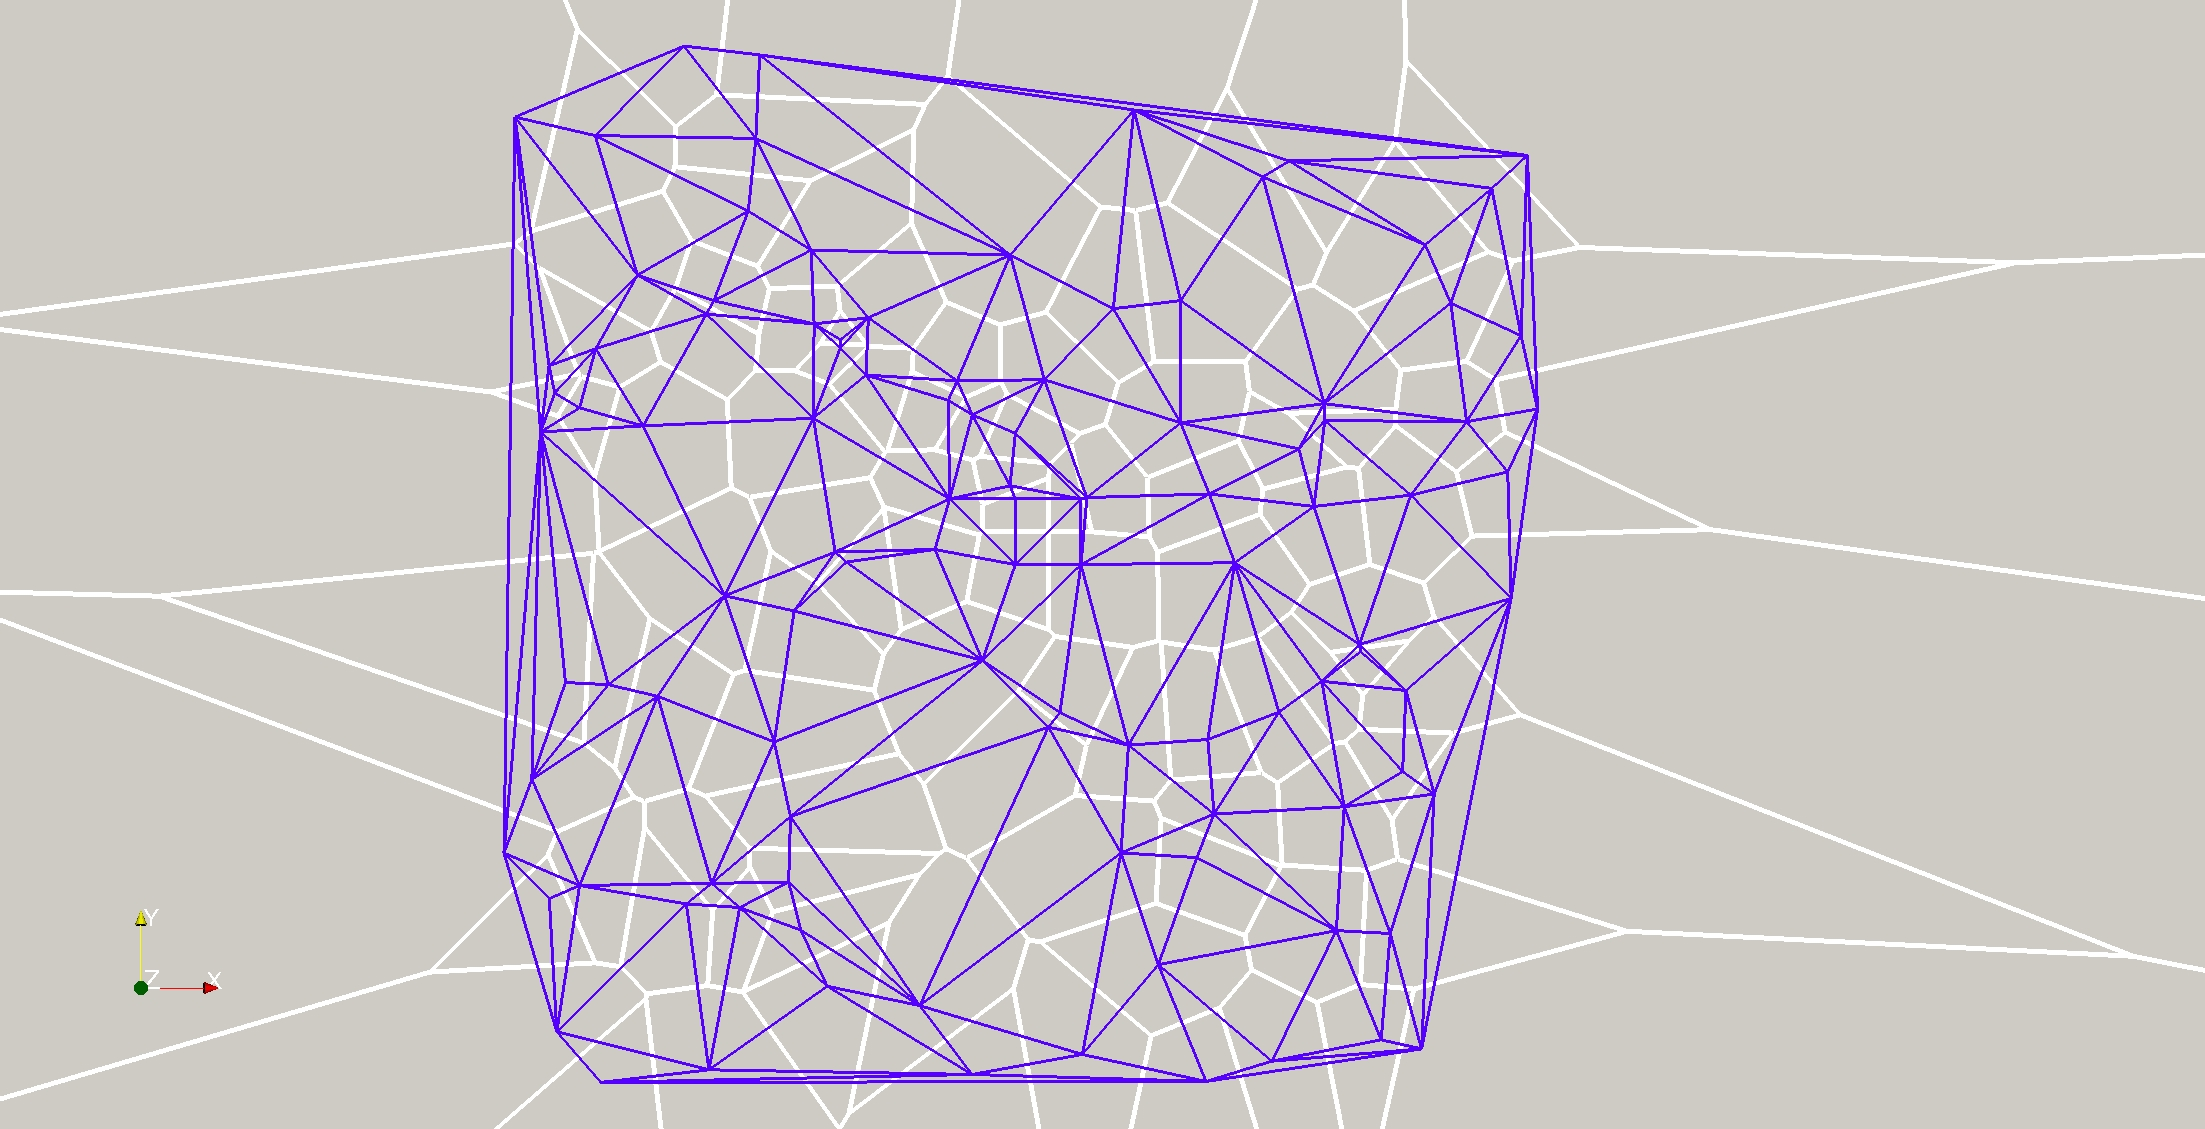
\includegraphics[scale=0.18, viewport=450 30 1630 1300, clip]{duality.jpg}
\end{center}
\end{Energie}

\subsection{Travail effectué}
\begin{Energie}{Première étude bibliographique}
\bibliographystyle{plain}
\begin{btSect}{doc.bib}
\btPrintCited
\btPrintNotCited
\end{btSect}
\label{biblio}
\end{Energie}

\usetikzlibrary {shapes.geometric}
\begin{Energie}{Bibliothèque logicielle programmée (C++)}
\begin{center}

\begin{onlyenv}<1>
\begin{tikzpicture}[fill=blue!20]
%\draw[help lines] (-1,-2) grid (6,3);
\path (0,0)
(10,0) node(c) [rectangle,draw,fill] {GeometricCore}
(5,0) node(d) [rectangle,draw,fill] {MeshCore}
(2,2) node(e) [rectangle,draw,fill] {MeshIO}
(2,0) node(f) [rectangle,draw,fill] {Delaunay}
(2,-2) node(g) [rectangle,draw,fill] {Voronoi};

\draw[thick, ->] (d) |- (c);
\draw[thick,->] (e) -- (d) ;
\draw[thick,->] (f) -- (d) ;
\draw[thick,->] (g) -- (d) ;
\draw[thick,blue,->] (f) .. controls +(down:1.5cm) .. (c);
\draw[thick,blue,->] (g.east) .. controls +(right:1.5cm) .. (c);
\end{tikzpicture}
\end{onlyenv}

\begin{onlyenv}<2>
\begin{tikzpicture}[fill=blue!20]
%\draw[help lines] (-1,-2) grid (6,3);
\path (0,0)
(10,0) node(c) [rectangle,draw,fill] {GeometricCore}
(5,0) node(d) [rectangle,draw,fill] {MeshCore}
(2,2) node(e) [rectangle,draw,fill] {MeshIO}
(2,0) node(f) [rectangle,draw,fill] {Delaunay}
(2,-2) node(g) [rectangle,draw,fill] {Voronoi}
(2,-4) node(h) [rectangle,draw,fill=red!30] {Test};
\draw[thick, ->] (d) |- (c);
\draw[thick,->] (h) -| +(-2,0) |- (f) ;
\draw[thick,->] (h) -| +(-2,0) |- (e) ;
\draw[thick,->] (h.north) -- (g) ;
\draw[thick,->] (h.east) -- (d) ;
\draw[thick,->] (h.east) -- (c) ;
\draw[thick,->] (e) -- (d) ;
\draw[thick,->] (f) -- (d) ;
\draw[thick,->] (g) -- (d) ;
\draw[thick,blue,->] (f) .. controls +(down:1.5cm) .. (c);
\draw[thick,blue,->] (g.east) .. controls +(right:1.5cm) .. (c);
\end{tikzpicture}
\end{onlyenv}
%\label{archi}

Architecture du projet (sous QtCreator)
\end{center}
\end{Energie}

\begin{Energie}{Structure en demi-arêtes}
\begin{center}
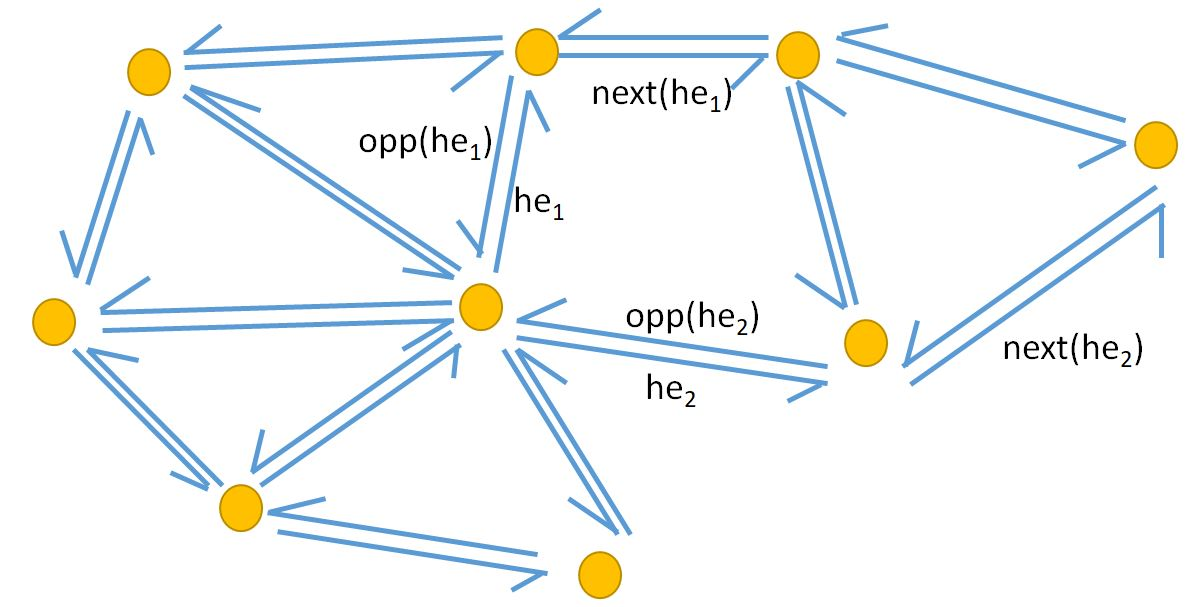
\includegraphics[scale=0.4]{../pictures/halfEdge.jpg}

Légende :

flèche bleue : demi-arête, rond : sommet, \texttt{opp} : demi-arête opposée, \texttt{next} : demi-arête suivante
\end{center}
\end{Energie}

\begin{Energie}{Algorithmes de génération de maillages}

\begin{itemize}
\item<1-4> gift-wrapping
\item<1,5,6> Bowyer-Watson
\end{itemize}
\begin{onlyenv}<2>
\begin{center}
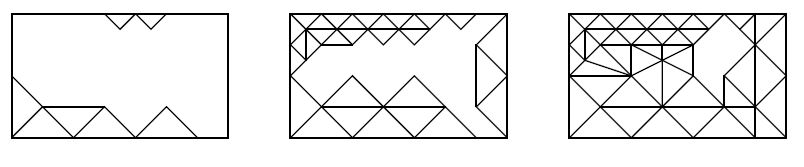
\includegraphics[scale=0.7]{advancingFront.jpg}
\\Figure 1.7 de la source \cite{delnotes} : principe d'une méthode d'avancée de front
\end{center}
\end{onlyenv}
\begin{onlyenv}<3>
\begin{center}
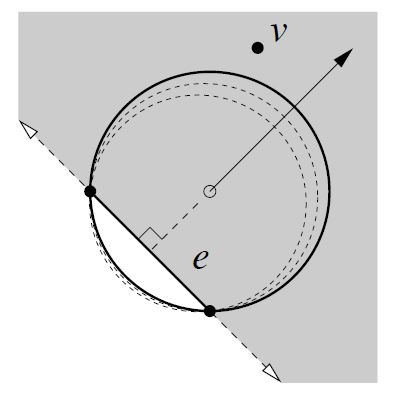
\includegraphics[scale=0.5]{giftWrappingStep.jpg}
\\Figure 3.11 de la source \cite{delnotes} : étape de finition d'une arête pour le \emph{gift-wrapping}
\end{center}
\end{onlyenv}
\begin{onlyenv}<4>\vspace{1cm}
Complexité en $\mathcal{O}(n^{2}m)$ avec $n$ le nombre de sommets et $m$ le nombre de segments contraintes
\end{onlyenv}

\begin{onlyenv}<5>
\begin{center}
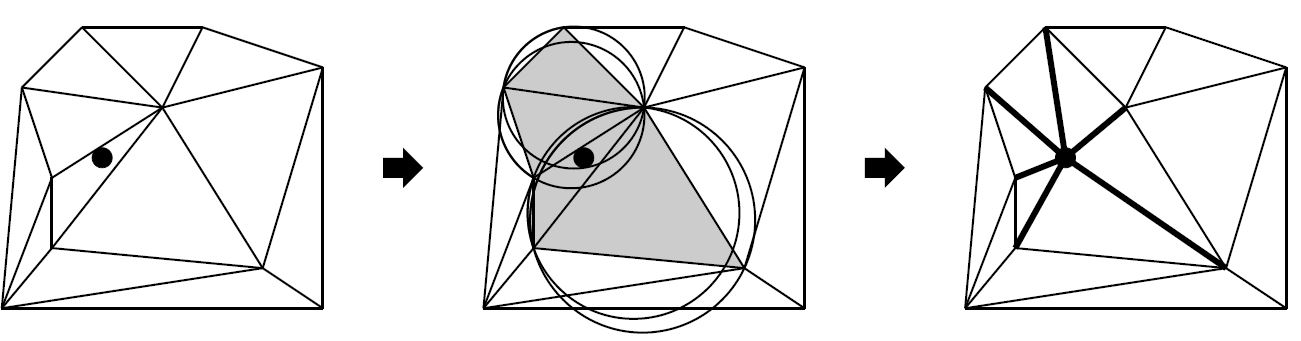
\includegraphics[scale=0.5]{bowyerWatson.jpg}
\\Figure 3.3 de la source \cite{delnotes} : algorithme de Bowyer-Watson
\end{center}
\end{onlyenv}
\begin{onlyenv}<6>\vspace{1cm}
Complexité en $\mathcal{O}(n\log(n))$ avec $n$ le nombre de sommets
\end{onlyenv}

\end{Energie}

\begin{Energie}{Graphe d'incidences}
\begin{center}
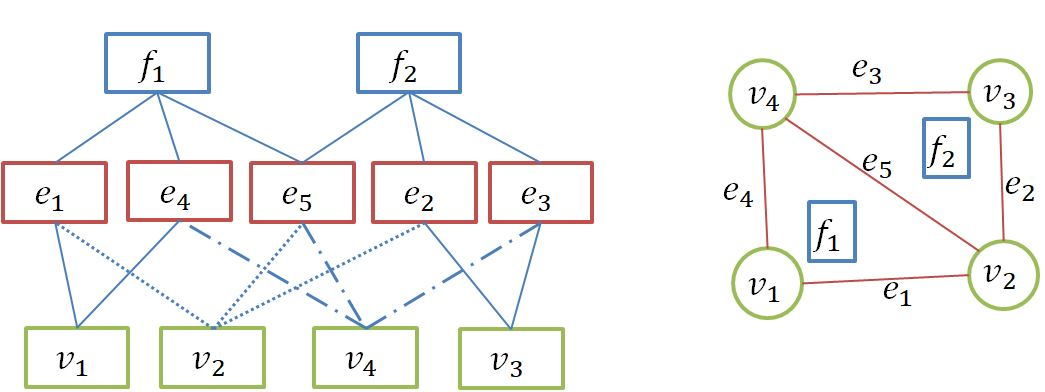
\includegraphics[scale=0.45]{adjacencies.jpg}
\end{center}
\end{Energie}

\begin{Energie}{Seconde étude bibliographique}\setbeamertemplate{itemize subitem}[square]

Elle concerne

\begin{itemize}
\item des structures de données représentant des maillages 3D polyédriques :
\begin{itemize}
\item demi-arêtes
\item cartes combinatoires
\item $\mathcal{G}$-cartes
\item $n$-cartes
\end{itemize}
\item des méthodes de génération de maillages polyédriques pour des simulations en géosciences :
\begin{itemize}
\item par résolution de problèmes d'optimisation
\item par des algorithmes de raffinement
\end{itemize}
\end{itemize}
\end{Energie}

\subsection{Résultats}
\begin{Energie}{Résultats}
\begin{itemize}
\item structure en demi-arêtes pour maillages bidimensionnels
\item algorithmes de génération de maillages
\item maillages polygonaux (Delaunay, Voronoï) exportés dans $3$ formats (OBJ, PLY, XDMF), de domaines du plan, convexes ou non
\item temps de calcul diminué grâce à la structure d'arbre quaternaire
\end{itemize}
\end{Energie}

\begin{Energie}{\normalsize Exemple de complexe linéaire par morceaux à mailler}
\begin{center}
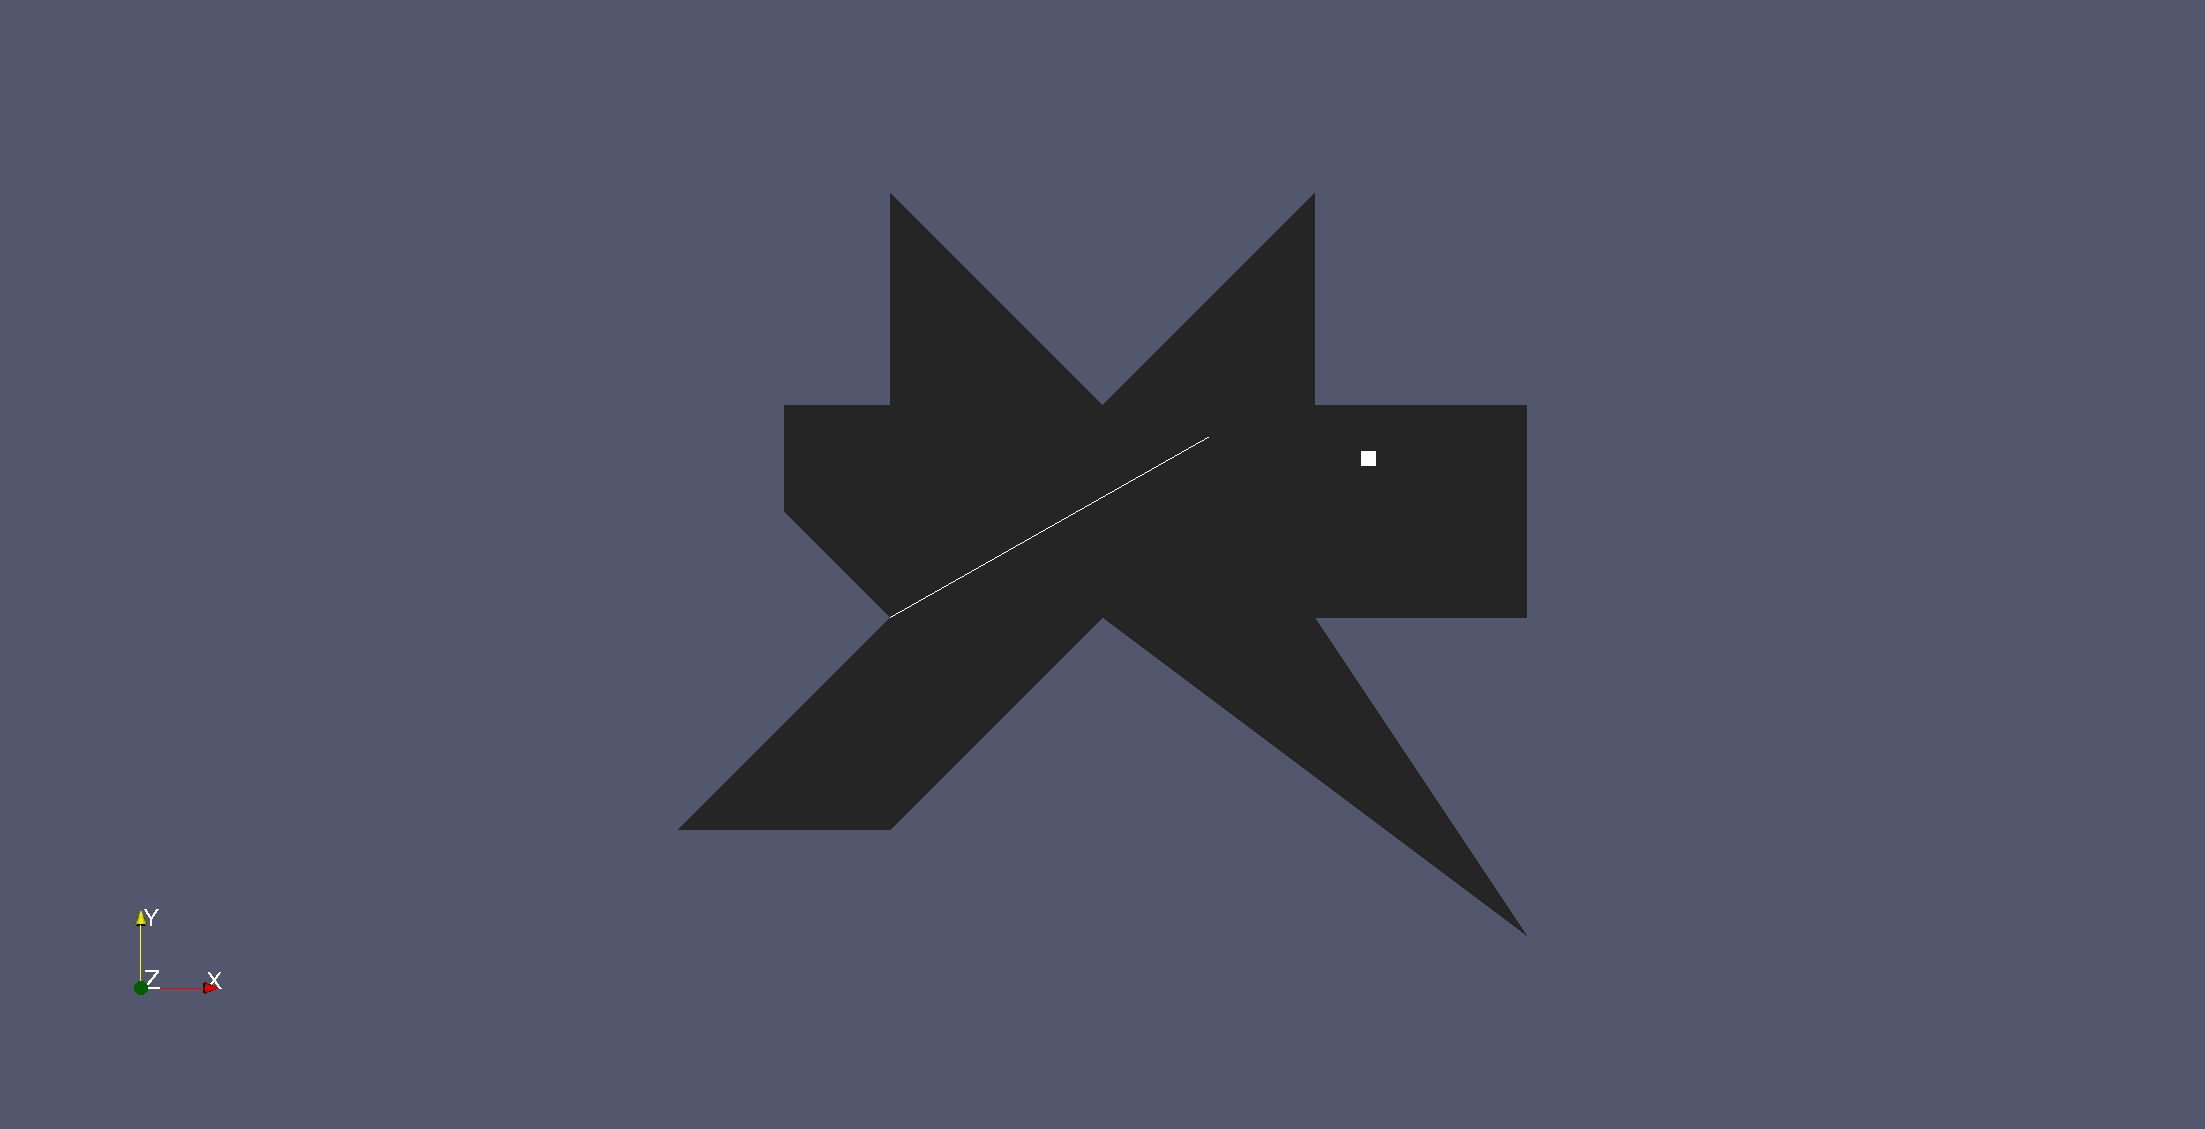
\includegraphics[scale=0.18, viewport=430 0 1800 1129, clip]{odd_plc.jpg}
\end{center}
\end{Energie}

\begin{Energie}{\normalsize Triangulation de Delaunay contrainte correspondante}
\begin{center}
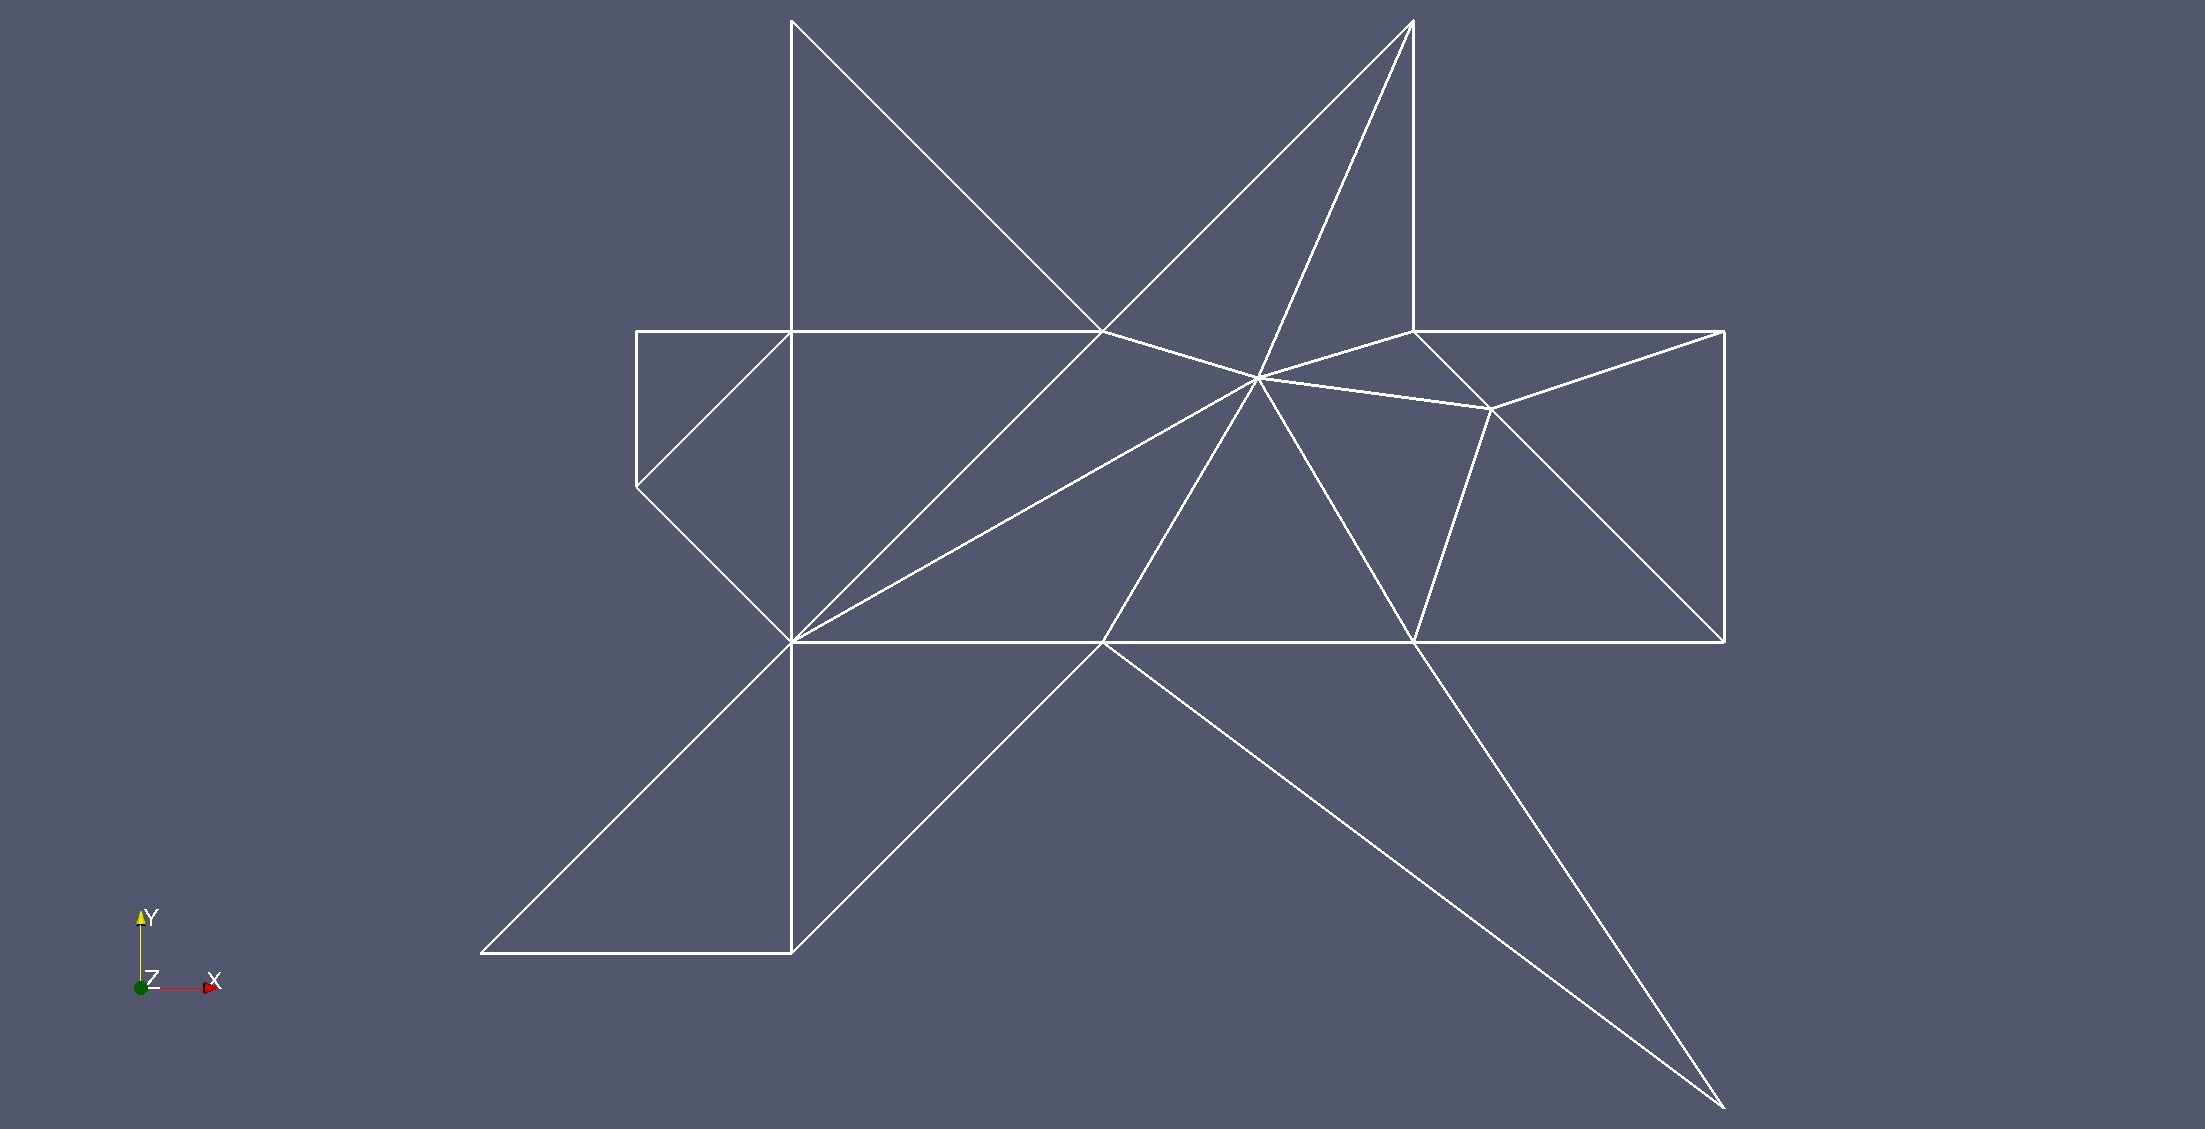
\includegraphics[scale=0.18, viewport=430 0 1800 1129, clip]{odd_cdt.jpg}
\end{center}
\end{Energie}

\begin{Energie}{\normalsize Un autre complexe linéaire par morceaux}
\begin{center}\vspace{-1cm}
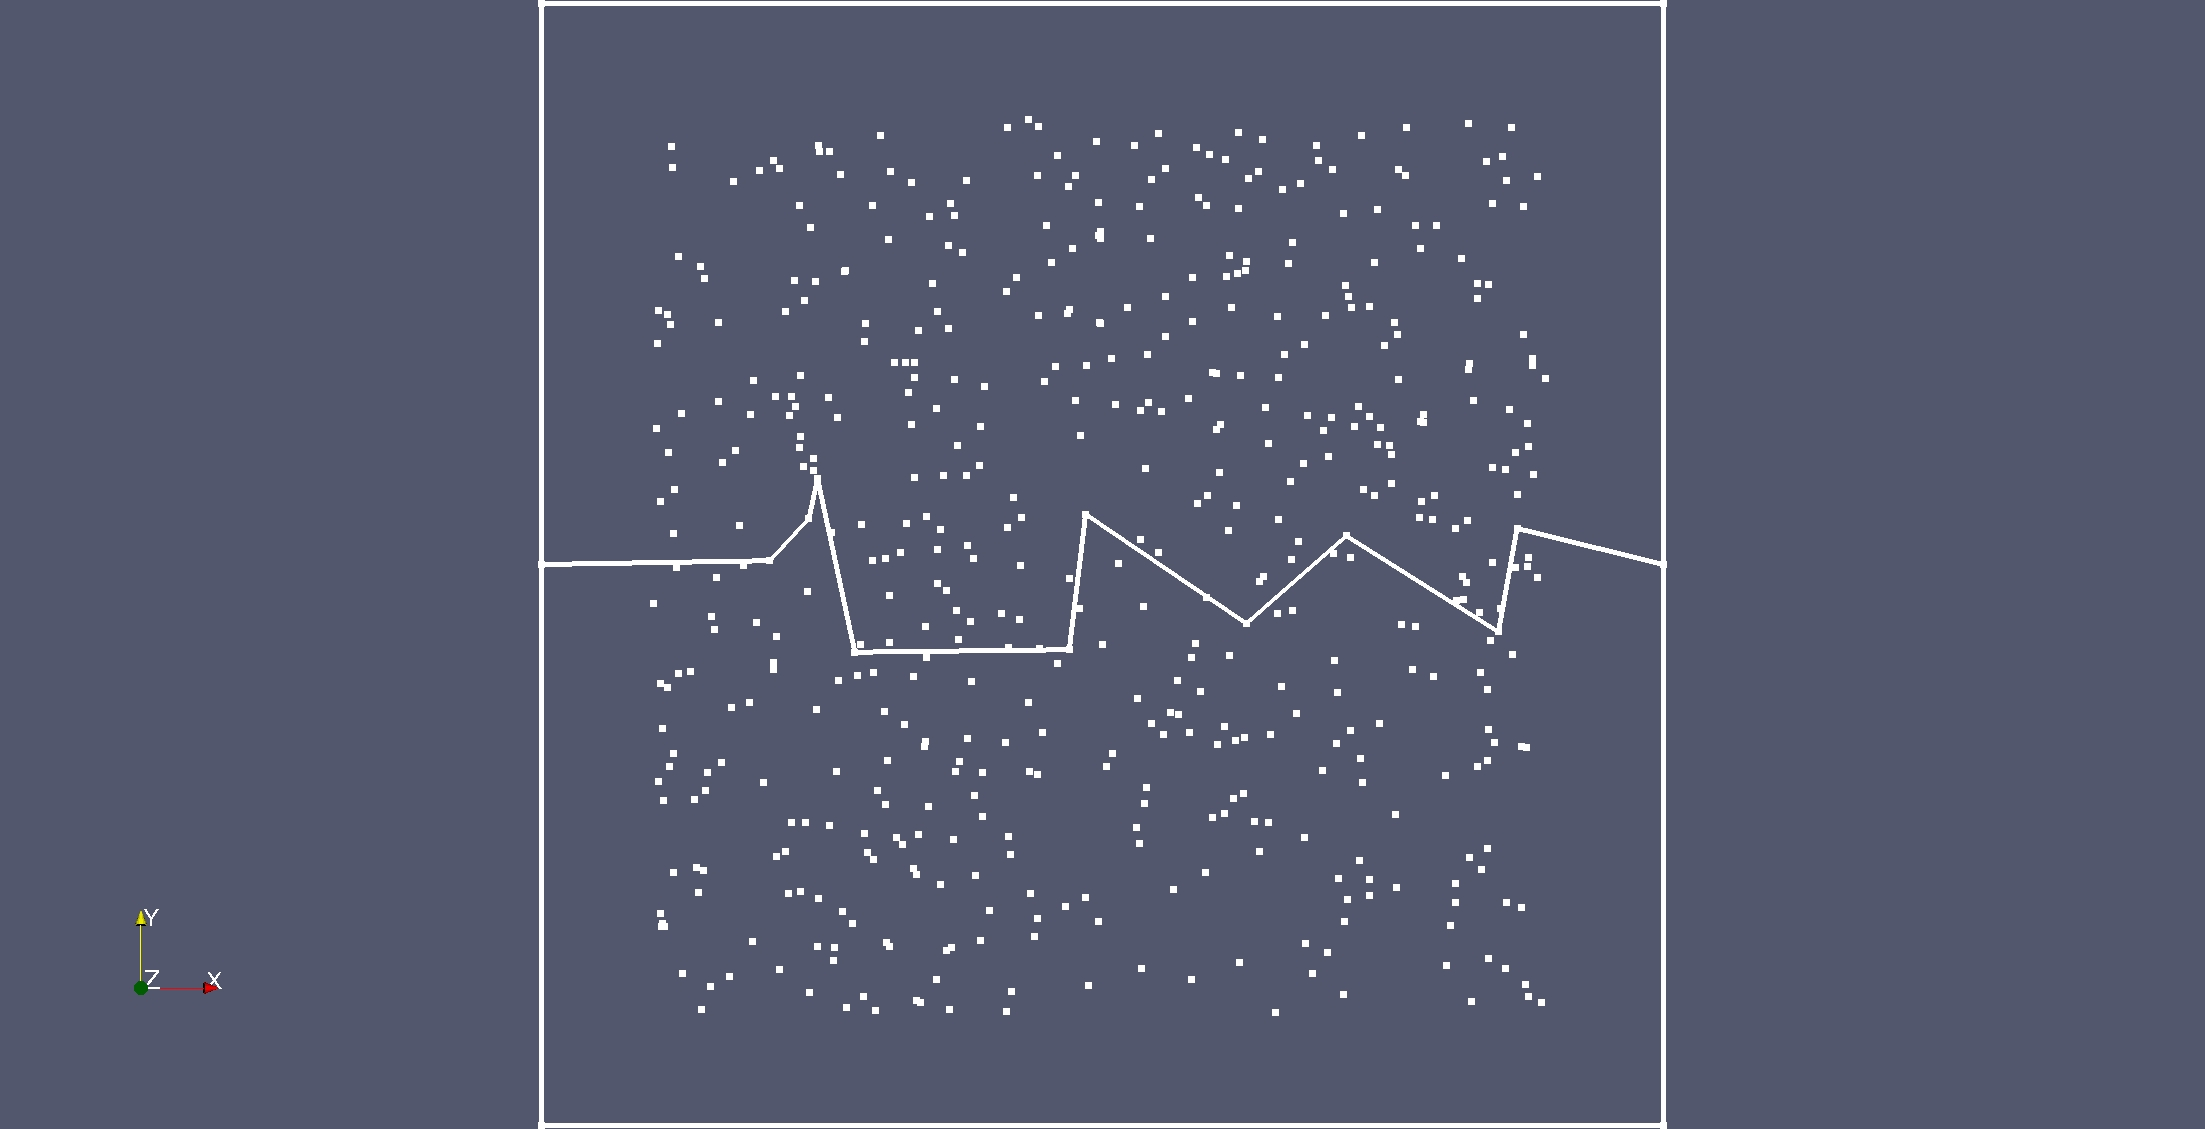
\includegraphics[scale=0.18, viewport=500 0 1700 1300, clip]{plc.jpg}
\end{center}
\end{Energie}

\begin{Energie}{\normalsize Triangulation de Delaunay correspondante}
\begin{center}\vspace{-1cm}
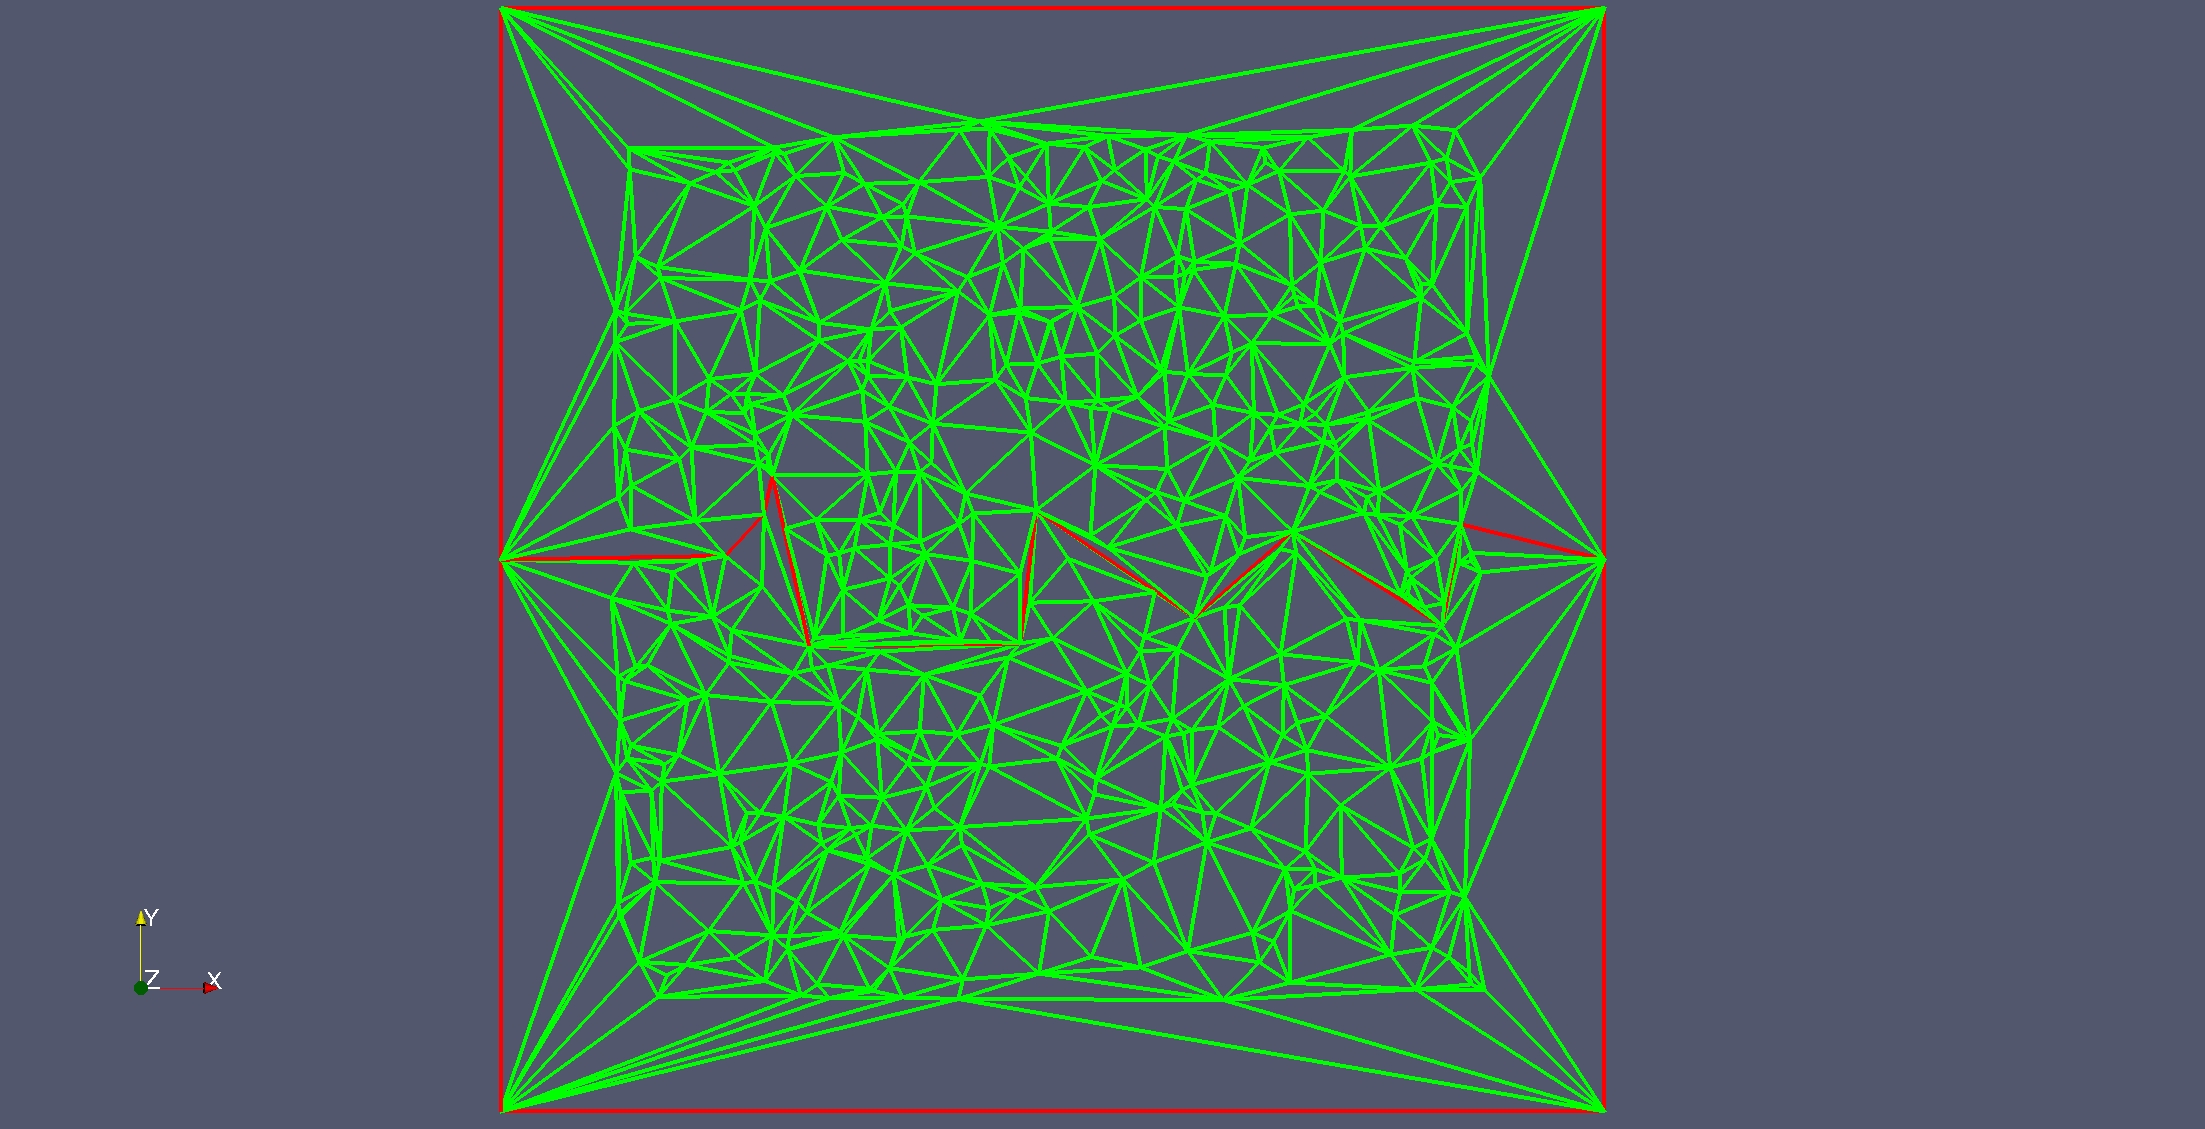
\includegraphics[scale=0.18, viewport=480 0 1630 1300, clip]{interfaceInSquare.jpg}
\end{center}
\end{Energie}

\begin{Energie}{\normalsize Diagramme de Voronoï correspondant}
\begin{center}\vspace{-1cm}
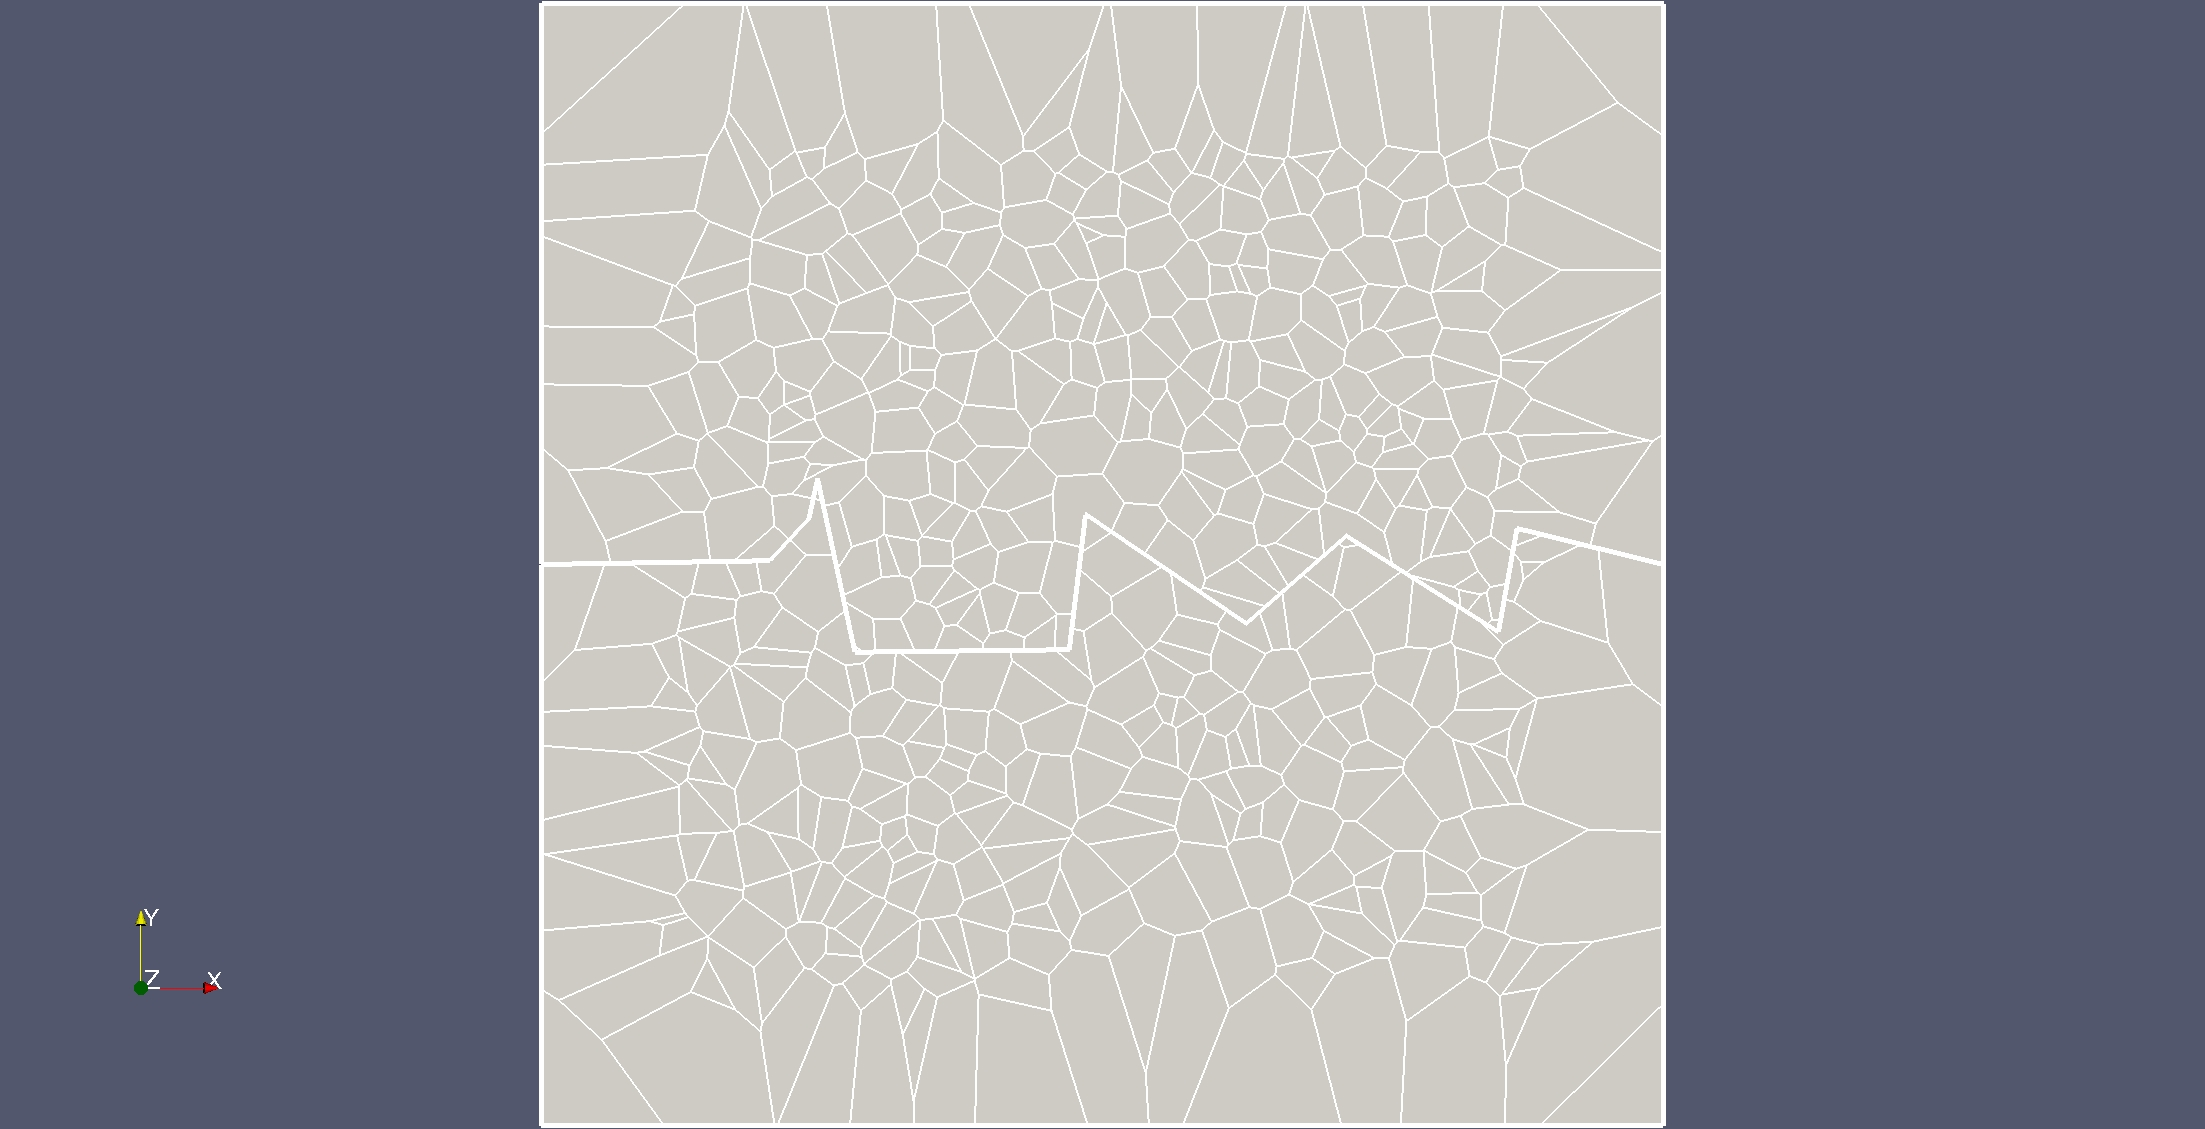
\includegraphics[scale=0.18, viewport=500 0 1700 1300, clip]{extended_vor.jpg}
\end{center}
\end{Energie}


\subsection{Difficultés}

\begin{Energie}{Difficultés}
\begin{itemize}
\item différence entre théorie et pratique (arithmétique flottante)
\item conventions disparates des logiciels de visualisations (Paraview, CloudCompare, MeshLab)
\item existence de nombreux cas particuliers difficiles à couvrir avec des tests unitaires (intersections$\dots$)
\end{itemize}
\end{Energie}

\section{Conclusion}
\begin{Energie}{Conclusion}\setbeamertemplate{itemize subitem}[ball]

Ce stage m'a permis de

\begin{itemize}
\item<1-> découvrir des concepts en génération de maillages pour les géosciences
\item<2-> de préparer la thèse qui suit : 
\begin{itemize}
\item<3-> difficultés algorithmiques
\item<4-> erreurs à ne pas reproduire (code, théorie)
\item<5-> bibliographie
\end{itemize}
\end{itemize}
\end{Energie}

\makeByeSlide

\begin{Energie}{\small Bibliographie additionnelle}

{\tiny
\begin{btSect}{additional.bib}
\btPrintNotCited
\end{btSect}}
\end{Energie}

\begin{Energie}{\small Sources des modèles géologiques}

{\fontsize{10}{12}\selectfont
\begin{btSect}{models.bib}
\btPrintNotCited
\btPrintCited
\end{btSect}}
\end{Energie}


%annexes
\begin{Energie}{Arête localement Delaunay}
\begin{center}
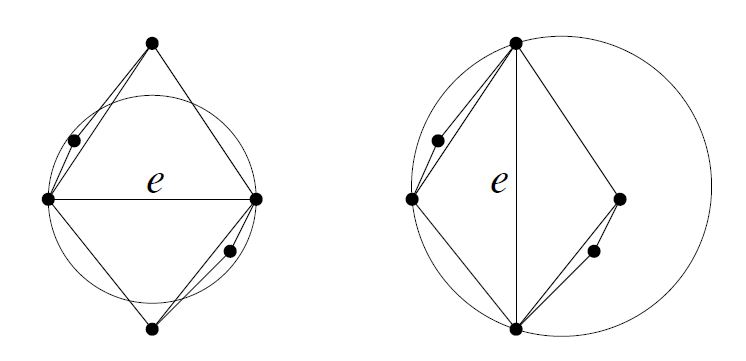
\includegraphics[scale=0.6]{locDel.jpg}
\\figure 2.7 de la source \cite{delnotes}
\end{center}
\end{Energie}

\begin{Energie}{Quadtree : boîtes englobantes}
\begin{center}
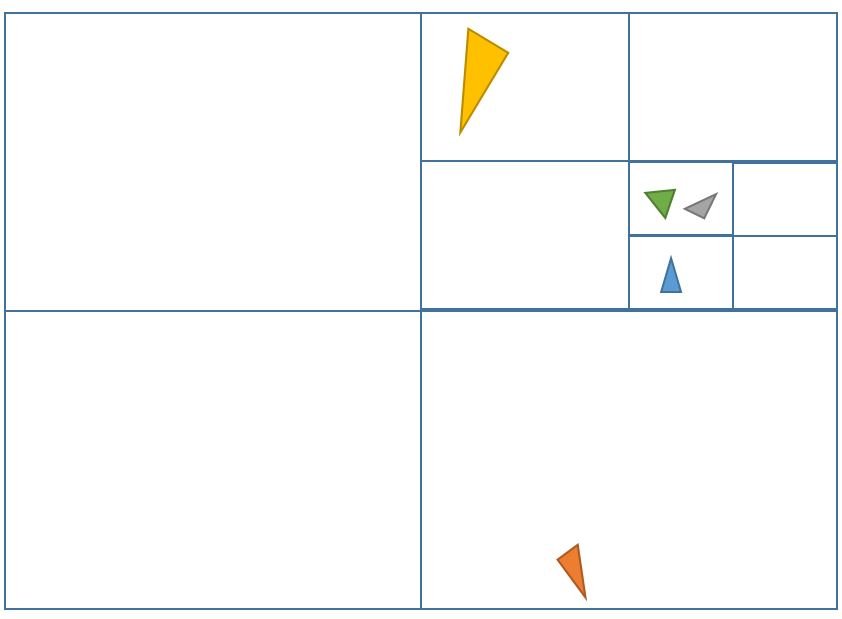
\includegraphics[scale=0.5]{boundingBoxes.jpg}
\end{center}
\end{Energie}

\begin{Energie}{Quadtree : structure d'arbre}

\begin{columns}[c]
\column{4cm}
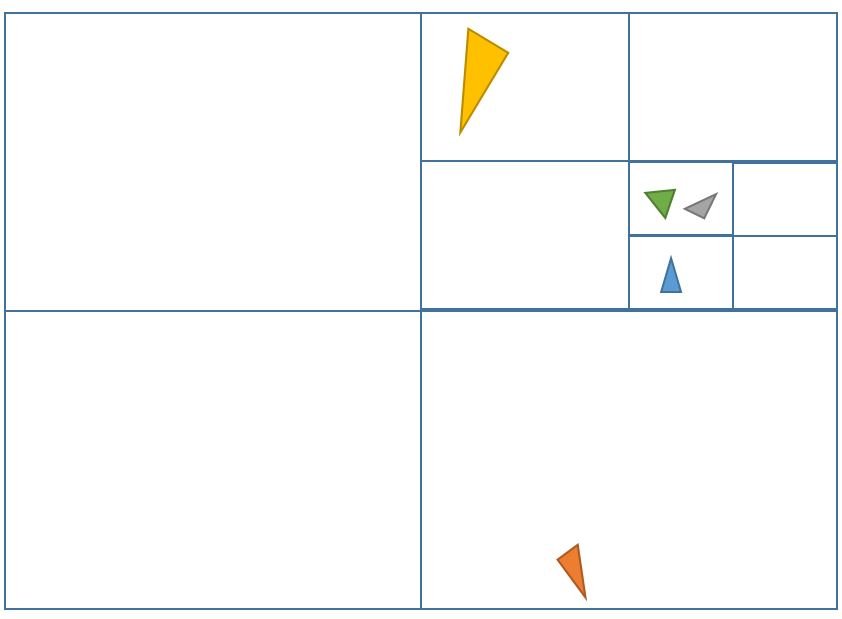
\includegraphics[scale=0.28]{boundingBoxes.jpg}
\column{8cm}
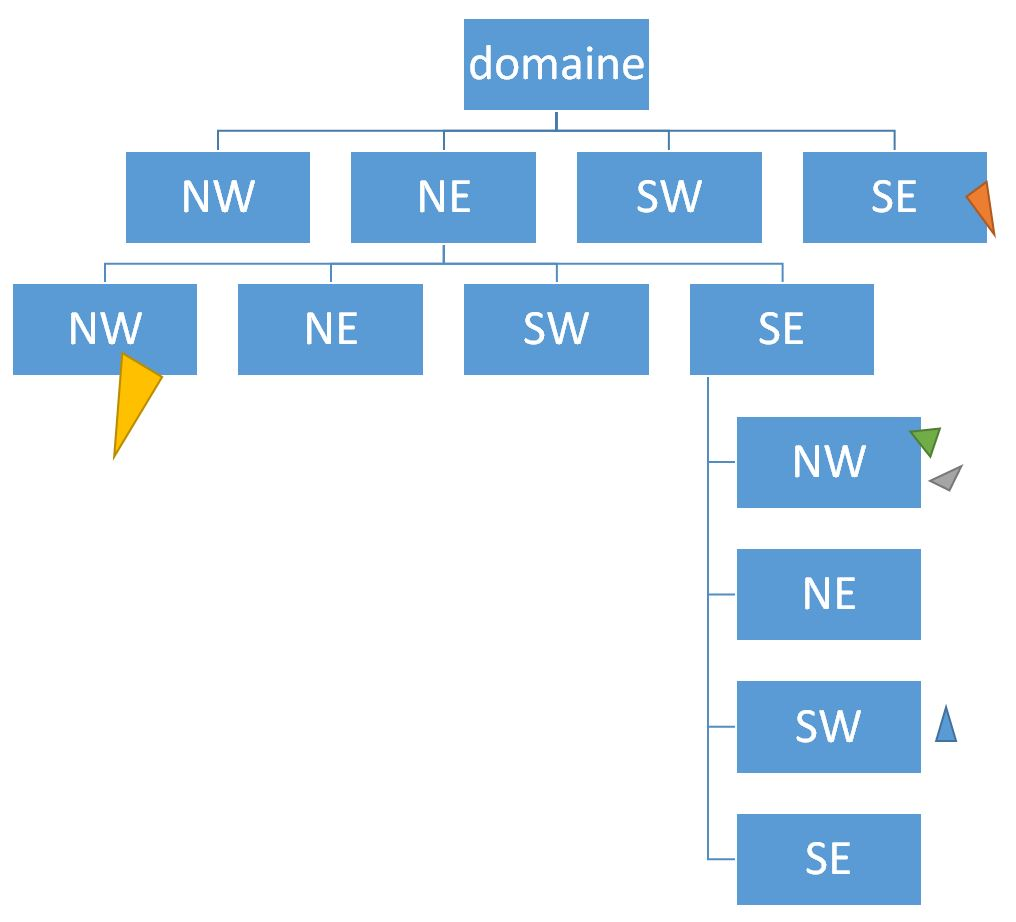
\includegraphics[scale=0.35]{quadtree.jpg}
\end{columns}
\end{Energie}

\end{document}
